
\tikzset{every picture/.style={line width=0.75pt}} %set default line width to 0.75pt        

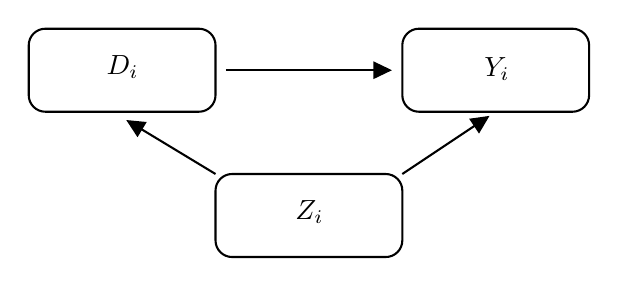
\begin{tikzpicture}[x=0.75pt,y=0.75pt,yscale=-1,xscale=1]
%uncomment if require: \path (0,361); %set diagram left start at 0, and has height of 361

%Rounded Rect [id:dp7232682276583055] 
\draw   (230,168) .. controls (230,163.58) and (233.58,160) .. (238,160) -- (312,160) .. controls (316.42,160) and (320,163.58) .. (320,168) -- (320,192) .. controls (320,196.42) and (316.42,200) .. (312,200) -- (238,200) .. controls (233.58,200) and (230,196.42) .. (230,192) -- cycle ;

%Rounded Rect [id:dp7900793201983274] 
\draw   (320,98) .. controls (320,93.58) and (323.58,90) .. (328,90) -- (402,90) .. controls (406.42,90) and (410,93.58) .. (410,98) -- (410,122) .. controls (410,126.42) and (406.42,130) .. (402,130) -- (328,130) .. controls (323.58,130) and (320,126.42) .. (320,122) -- cycle ;

%Rounded Rect [id:dp49000656757418604] 
\draw   (140,98) .. controls (140,93.58) and (143.58,90) .. (148,90) -- (222,90) .. controls (226.42,90) and (230,93.58) .. (230,98) -- (230,122) .. controls (230,126.42) and (226.42,130) .. (222,130) -- (148,130) .. controls (143.58,130) and (140,126.42) .. (140,122) -- cycle ;

%Straight Lines [id:da16218237230483512] 
\draw    (320,160) -- (359.5,133.66) ;
\draw [shift={(362,132)}, rotate = 146.31] [fill={rgb, 255:red, 0; green, 0; blue, 0 }  ][line width=0.08]  [draw opacity=0] (8.93,-4.29) -- (0,0) -- (8.93,4.29) -- cycle    ;
%Straight Lines [id:da880895933850384] 
\draw    (230,160) -- (189.57,135.55) ;
\draw [shift={(187,134)}, rotate = 31.16] [fill={rgb, 255:red, 0; green, 0; blue, 0 }  ][line width=0.08]  [draw opacity=0] (8.93,-4.29) -- (0,0) -- (8.93,4.29) -- cycle    ;
%Straight Lines [id:da6515543213351532] 
\draw    (235,110) -- (312,110) ;
\draw [shift={(315,110)}, rotate = 180] [fill={rgb, 255:red, 0; green, 0; blue, 0 }  ][line width=0.08]  [draw opacity=0] (8.93,-4.29) -- (0,0) -- (8.93,4.29) -- cycle    ;

% Text Node
\draw (176,101.4) node [anchor=north west][inner sep=0.75pt]    {$D_{i}$};
% Text Node
\draw (267,171.4) node [anchor=north west][inner sep=0.75pt]    {$Z_{i}$};
% Text Node
\draw (358,102.4) node [anchor=north west][inner sep=0.75pt]    {$Y_{i}$};


\end{tikzpicture}